\documentclass[a4paper]{article}

\usepackage[per-mode=symbol,separate-uncertainty=true]{siunitx}
\usepackage{amsmath}
\usepackage{float}
\usepackage{graphicx}
\usepackage[a4paper,top=3cm,bottom=2cm,left=3cm,right=3cm,marginparwidth=1.75cm]{geometry}
\usepackage{mathtools}
\usepackage{subcaption}
\usepackage{xcolor}
\usepackage{xspace}
\usepackage{fancyhdr}
\usepackage{fancyvrb}
\usepackage{verbatimbox}
\usepackage{hyperref}

\newcommand{\inv}{\texttt{INV\_X4}\xspace}
\newcommand{\ha}{\texttt{HA\_X1}\xspace}

\title{Digital Microelectronics 2018 \\ Final project report}
\author{Marco Andorno (247222)\\ Michele Caon (253027) \\ Matteo Perotti (251453)}

\begin{document}

% INTRO
\begin{center}

\thispagestyle{empty}

\textbf{\Large Digital Microelectronics}\\[1.0cm]
\textsc{\Large Politecnico di Torino}\\[0.5cm]
\textsc{\large Dipartimento di Elettronica e Telecomunicazioni}\\[1cm]

% TITLE
\huge \textbf{Final Project: \\}
\huge \textbf{Standard Cell layout of an inverter and a half-adder}

\end{center}

% AUTHORS
\vfill
\large
\begin{flushleft}
\makeatletter
\emph{Group 5:}\\
\@author \\
\vspace{1cm}
\normalsize Date: \today
\makeatother
\end{flushleft}

%\maketitle

\newpage

\pagestyle{fancy}
\lhead{}
\chead{}
\rhead{\leftmark}
\lfoot{\thepage}
\cfoot{}
\rfoot{}
\renewcommand{\headrulewidth}{0.3pt}
\renewcommand{\footrulewidth}{0.3pt}

% \tableofcontents
% \newpage

\section{Introduction}
\label{sec:intro}
The goal of this final project is to design and characterize two logic gates of a standard cell library. These are in particular an inverter whose transistors have width four times the minimum, and therefore a 4 times the minimum drive strength (\inv in the following), and a half adder with minimum drive strength (\ha in the following).

The design starts from the schematic drawing, using an available \texttt{.png} image as a reference. This schematic will be simulated as an initial condition. Then, the layout of the cell must be drawn and the parasitic elements must be extracted from it. Finally, those parasitics must be taken into account during the final characterization. These results necessary to fill in the Liberty file of the standard cell library, replacing the old ones.

The files generated by the software tools for these two gates are inside the following paths on the server:
\begin{equation*}
	\texttt{/home/md18.5/project/INV\_X4/}
\end{equation*}
and
\begin{equation*}
	\texttt{/home/md18.5/project/HAX1/}
\end{equation*}
while the current report file and the final Liberty files filled with the simulated timing parameters can be found in
\begin{equation*}
	\texttt{/home/md18.5/project/report\_files/}
\end{equation*}

Notice that all the produced material, like scripts, plots and the current report files, can be found in the following GitHub repository:
\begin{center}
	\url{https://github.com/mksoc/standard-cell-design}
\end{center}

\section{Inverter}

\subsection{Schematic}

\label{sec: inv_sch}
Starting from the schematic of the reference \texttt{.png} (figure \ref{fig:inv_png}), we copied it using Virtuoso Schematic Editor, obtaining the result shown in figure \ref{fig:inv_schematic}. Note that the four PMOS and NMOS transistors in parallel will be implemented as one large transistor in the layout, with the source/drain diffusions fingered.
\begin{figure}[H]
	\centering
	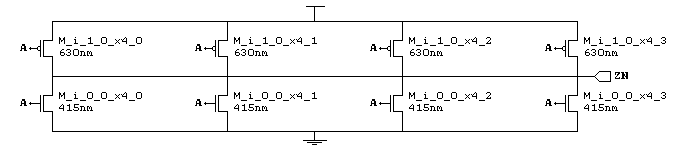
\includegraphics[width=1\linewidth]{../INV_X4/INV_X4.png}
	\caption{Reference schematic of the inverter}
	\label{fig:inv_png}
\end{figure}
\begin{figure}[H]
	\centering
	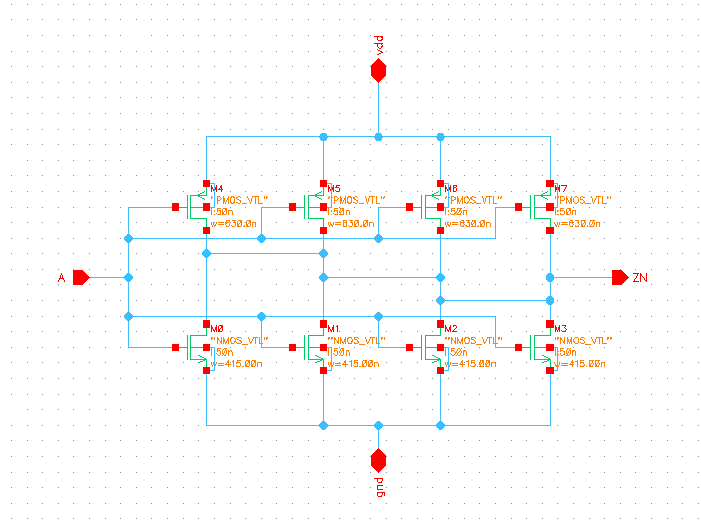
\includegraphics[width=\linewidth]{../INV_X4/INV_X4_schematic.png}
	\caption{Final schematic of \inv}
	\label{fig:inv_schematic}
\end{figure}

We then carried out some preliminary simulations using a test bench, to verify that the circuit worked correctly. We measured rise and fall times, as well as propagation delays, that will be compared with the actual characterization later on. We also measured the transfer characteristic, shown in figure \ref{fig:inv_tchar}.
\begin{figure}[H]
	\centering
	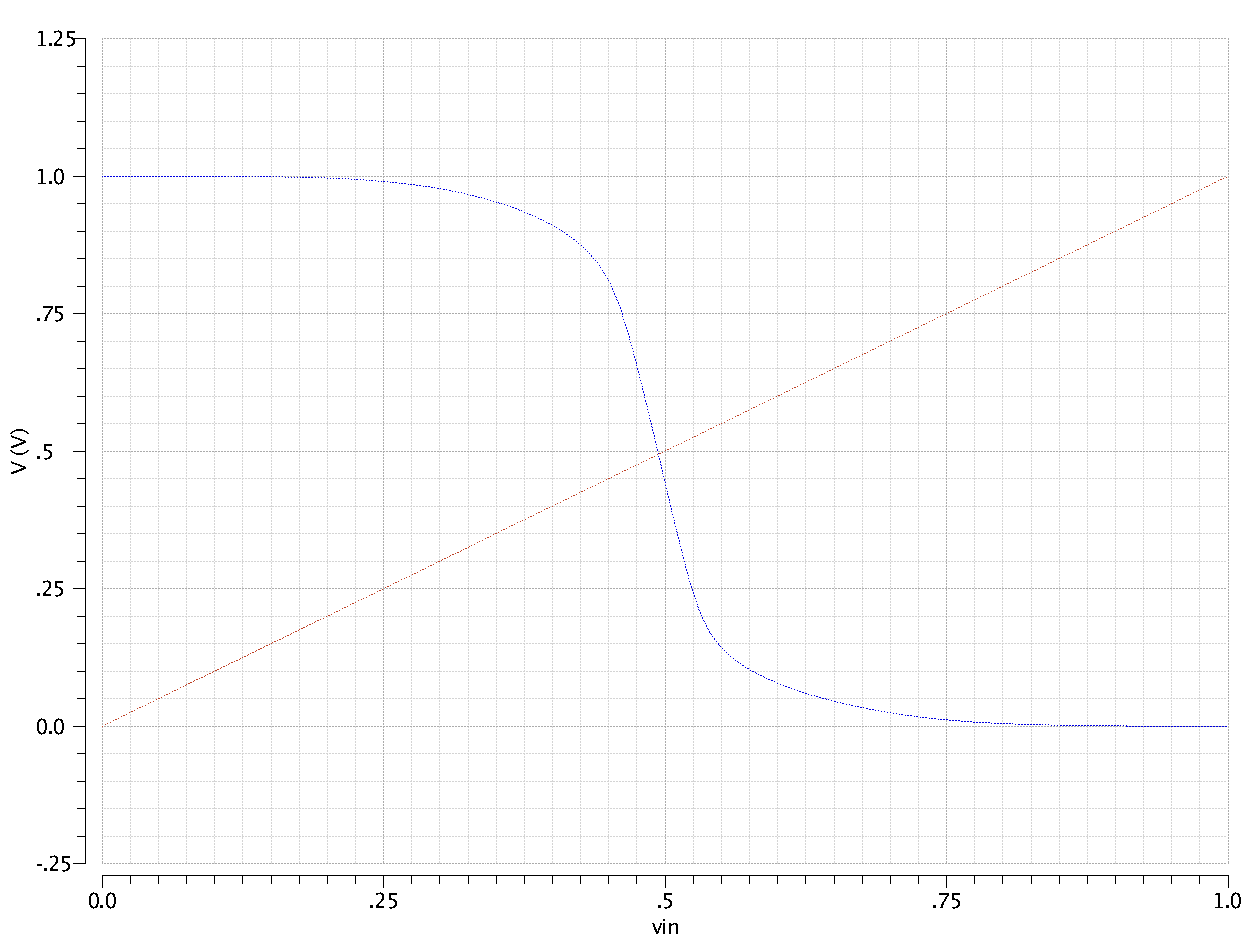
\includegraphics[width=.7\linewidth]{../INV_X4/INV_X4_transfer_char.pdf}
	\caption{Inverter transfer characteristic}
	\label{fig:inv_tchar}
\end{figure}

\subsection{Layout}
The final layout of \inv is shown in figure \ref{fig:inv_layout}. The main trick to note here is how we used transistor fingering extensively, by sharing as much as possible the source and drain diffusions between the different gates. This is generally done to reduce the total area of the standard cell, but in this case it was actually mandatory, because a single transistor large 4 times the minimum width would not fit inside the well height, at least for the PMOS pull-up network.
\begin{figure}[H]
	\centering
	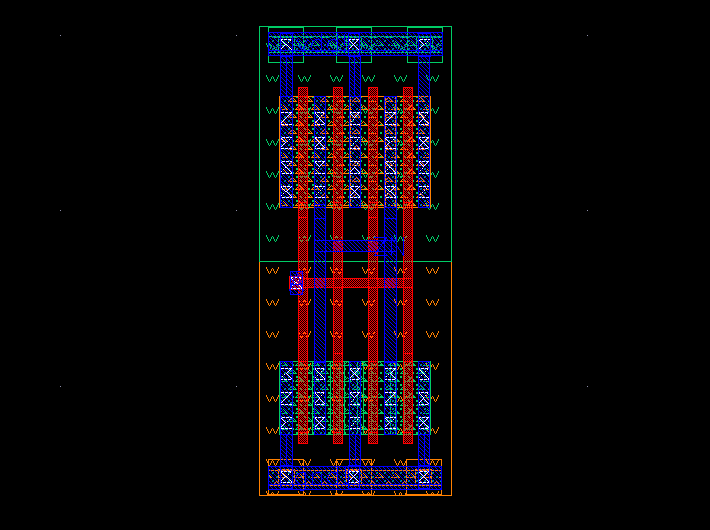
\includegraphics[width=\linewidth]{../INV_X4/INV_X4_layout.png}
	\caption{Layout of \inv}
	\label{fig:inv_layout}
\end{figure}

For PMOS transistors we were forced to finger four different transistor, while regarding the NMOS, probably, two fingered transistors with double width would have fit, but since the cell width would have been the same, we decided to go with four single width transistors anyway to improve symmetry.

Regarding pins, the output \texttt{ZN} did not cause any troubles and was placed on the rightmost metal strip connecting the drains of the PMOS and NMOS. As for the input \texttt{A}, instead, our first idea had been to place its via in the middle of the horizontal polysilicon strip, but then we noticed that this way the external connections to that pin would cross the \texttt{metal1} layer, thus requiring \texttt{metal2} to be used instead. So eventually we settled with placing the via for the input on the leftmost part of the polysilicon, avoiding any \texttt{metal1} crossing and also accurately refletting the topology of the schematic.

While developing the layout we ran the DRC tool many times to ensure all the design rules were met. After completing it we got the following final statement:
\newpage
\verbfilenobox[\small]{../INV_X4/INV_X4.drc.summary}
\newpage
Moreover, we compared the layout and the schematic netlists using LVS, that succeeded on the first try with its reassuring smiling smiley-face:
\verbfilenobox[\small]{../INV_X4/INV_X4.lvs.report}

Just a remark on the warning that says that nets \texttt{GND!} and \texttt{VDD!} are present in the layout but missing in the source (schematic). We tried to follow the steps of the laboratory sessions where the supply nets had the exclamation mark at the end in the layout view but not in the schematic one, and in fact we had no problems with this method for the \inv. However, we had a lot of issues for \ha when running LVS as it complained about missing power nets. We finally came to the conclusion that schematic and layout must have the exact same names for supply nets and that the exclamation mark can be avoided if the schematic does not exploit global nets to make the drawing cleaner and clearer. Even then, to this day it remains unclear why the inverter cell worked just as well with different names for power nets (disregarding this warning), while the half adder with the same setup caused so much trouble. We can only accept this and give in to the mighty secrets of Virtuoso.


\subsection{Characterization}
\label{sec: inv_char}
The first step toward the complete characterization of our logic gate was the extraction of the parasitic elements from the layout. To do this, we ran the PEX tool from the layout editor and got the following report as well as a complete new netlist that takes into account those parasitics in the schematic.
\verbfilenobox[\small]{../INV_X4/INV_X4.pex.report}

Then, we generated a new config view for our cell and linked it to the calibre view, which contained the aforementioned netlist with the parasitics. We then set up the old test bench to use this new view and ran the automatic simulations needed to compile the Liberty file and to perform the comparison with the schematic simulations.

In order to fill in the Liberty file faster we developed a Matlab script that converts the traces exported in \texttt{.csv} from Virtuoso into a suitable format for the \texttt{INV\_X4.lib} file. As already mentioned in section \ref{sec:intro}, this file can be found in the report directory on GitHub or on the server.
%\verbfilenobox[\small]{../INV_X4/INV_X4.lib}

We also developed another Matlab script to plot the results of the simulations, shown in the following figures.
\begin{figure}[H]
	\centering
	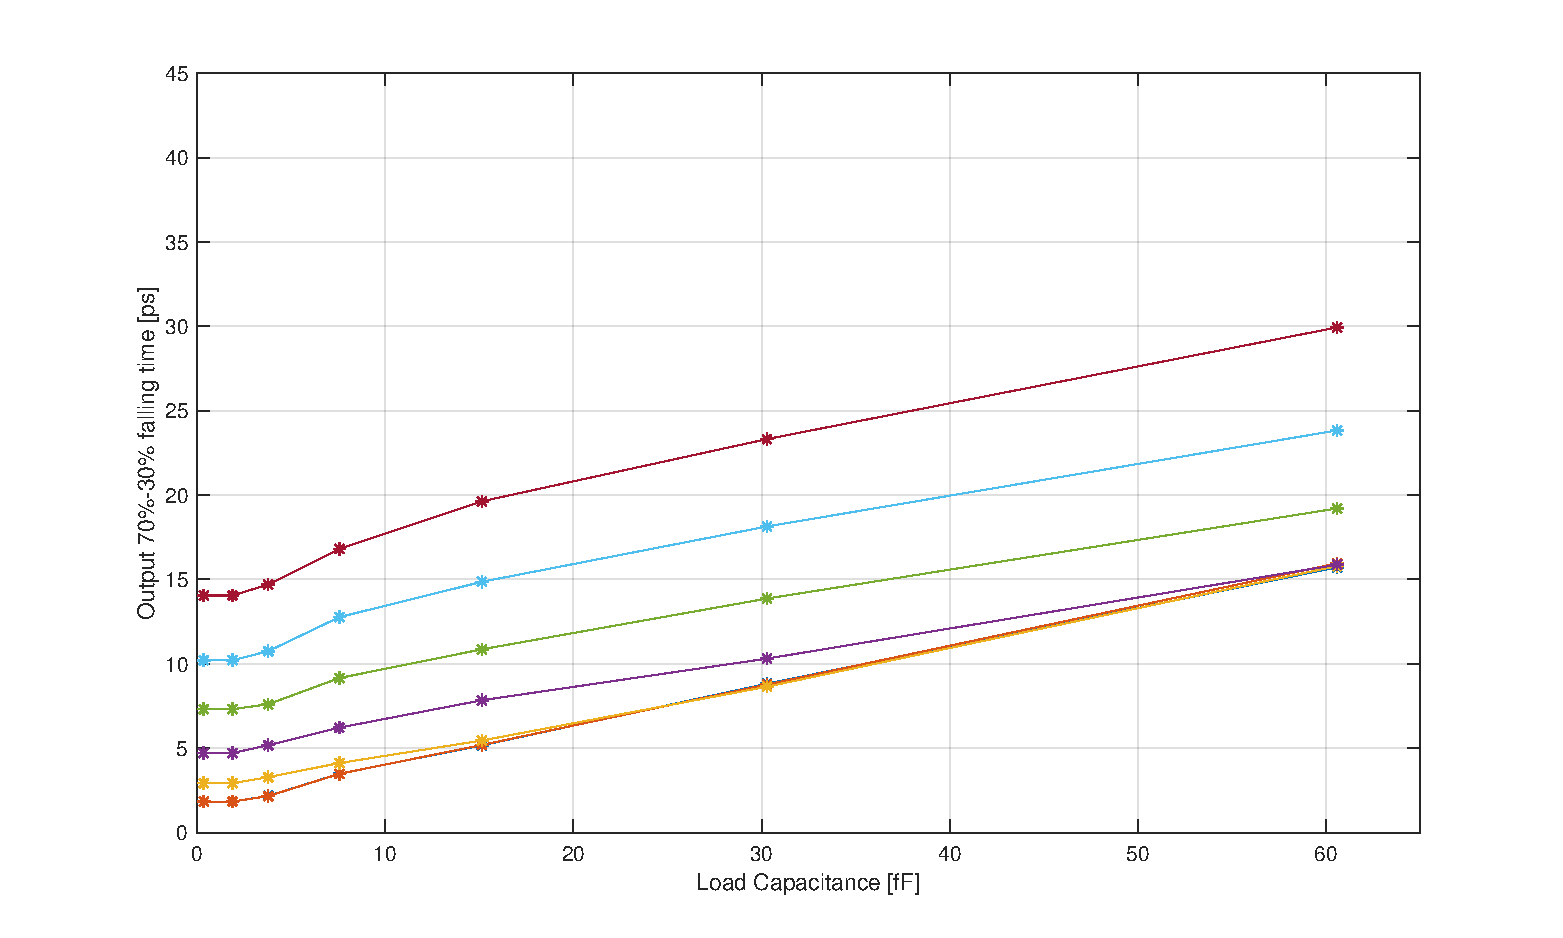
\includegraphics[width=\linewidth]{../INV_X4/simulations/t_F.pdf}
	\caption{Fall time vs load capacitance, higher curves are for longer input rise times.}
	\label{fig:inv_t_F}
\end{figure}
\begin{figure}[H]
	\centering
	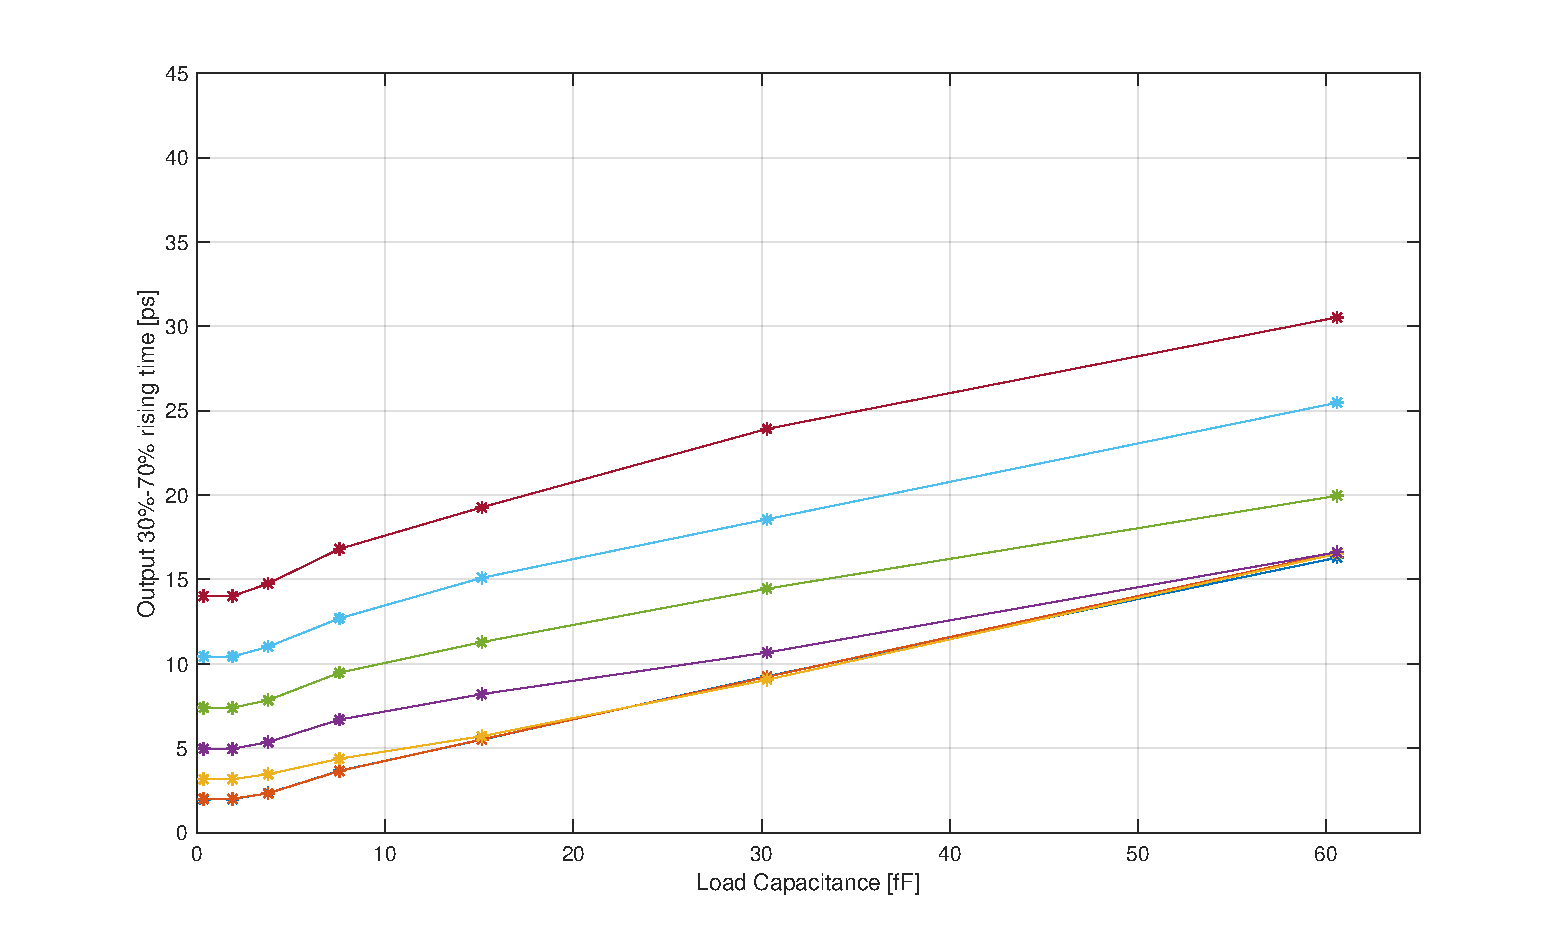
\includegraphics[width=\linewidth]{../INV_X4/simulations/t_R.pdf}
	\caption{Rise time vs load capacitance, higher curves are for longer input fall times.}
	\label{fig:inv_t_R}
\end{figure}
\begin{figure}[H]
	\centering
	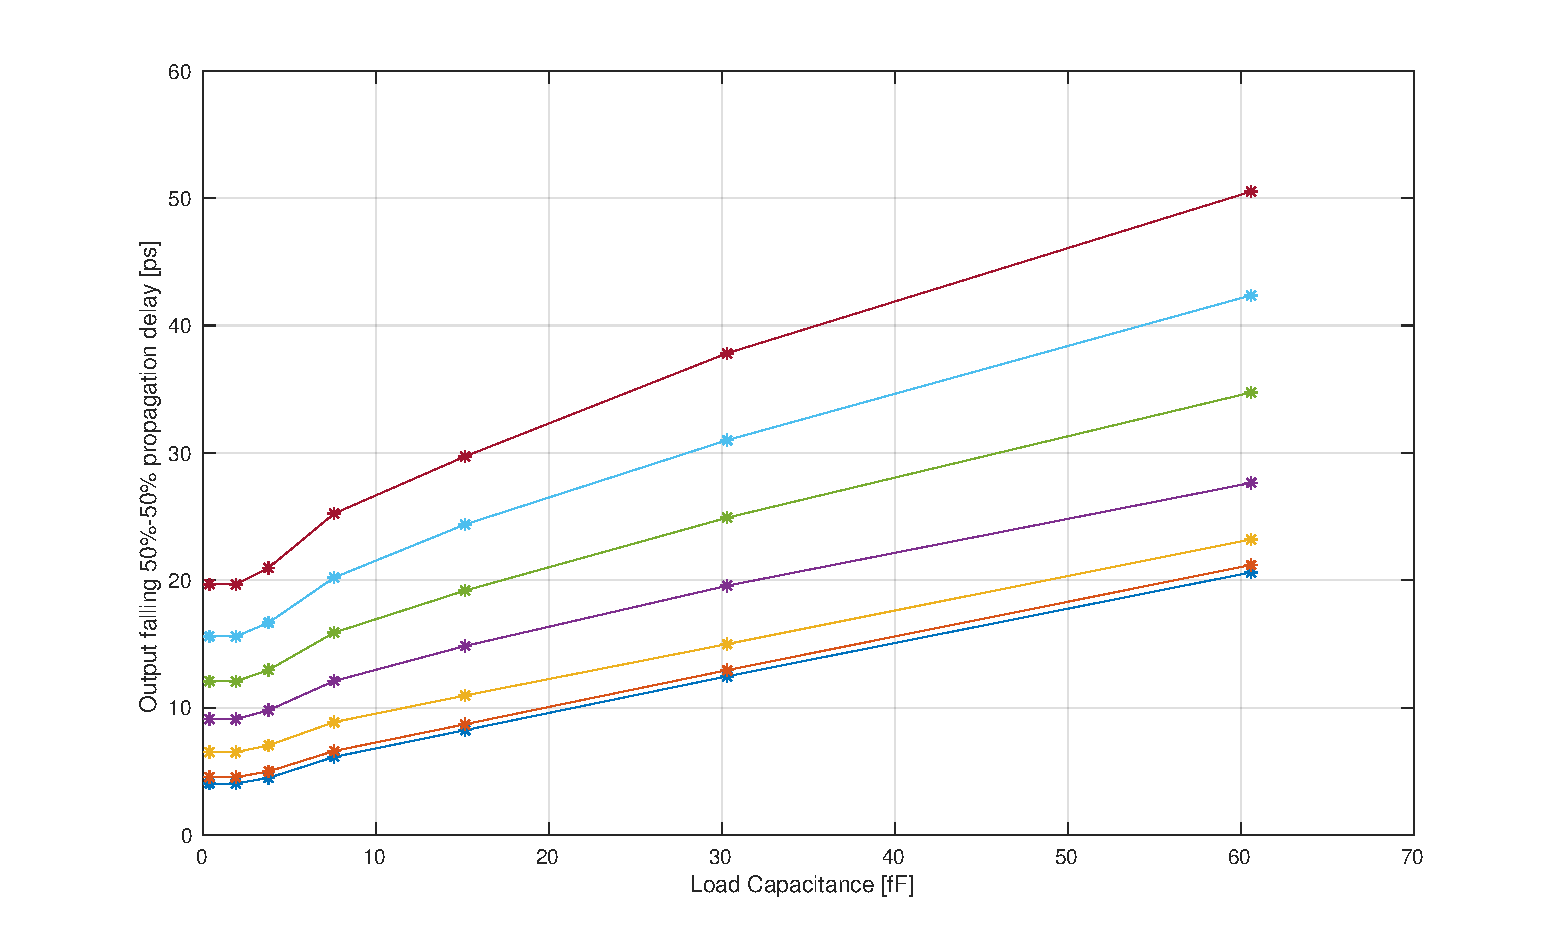
\includegraphics[width=\linewidth]{../INV_X4/simulations/tp_L.pdf}
	\caption{Output falling propagation delay vs load capacitance, higher curves are for longer input rise times.}
	\label{fig:inv_tp_L}
\end{figure}
\begin{figure}[H]
	\centering
	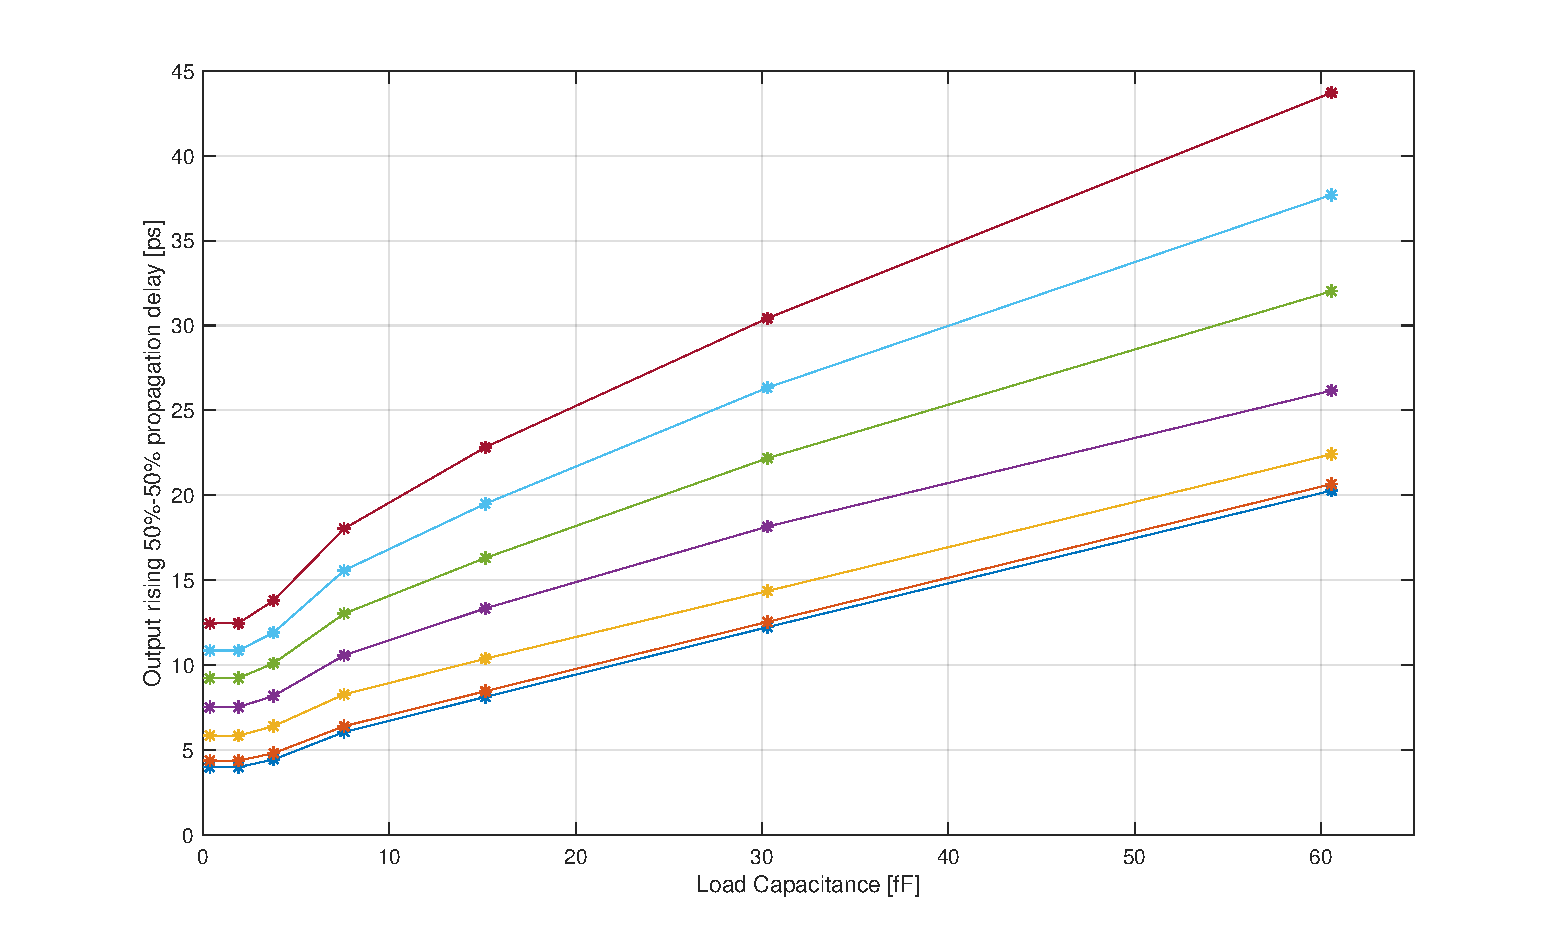
\includegraphics[width=\linewidth]{../INV_X4/simulations/tp_H.pdf}
	\caption{Output rising propagation delay vs load capacitance, higher curves are for longer input fall times.}
	\label{fig:inv_tp_H}
\end{figure}

We also compared these results with the simulation done with original schematic, computing the relative difference in the measured parameters for a given input delay (different input delay values gave similar results and thus were not meaningful to show).
\begin{figure}[H]
	\centering
	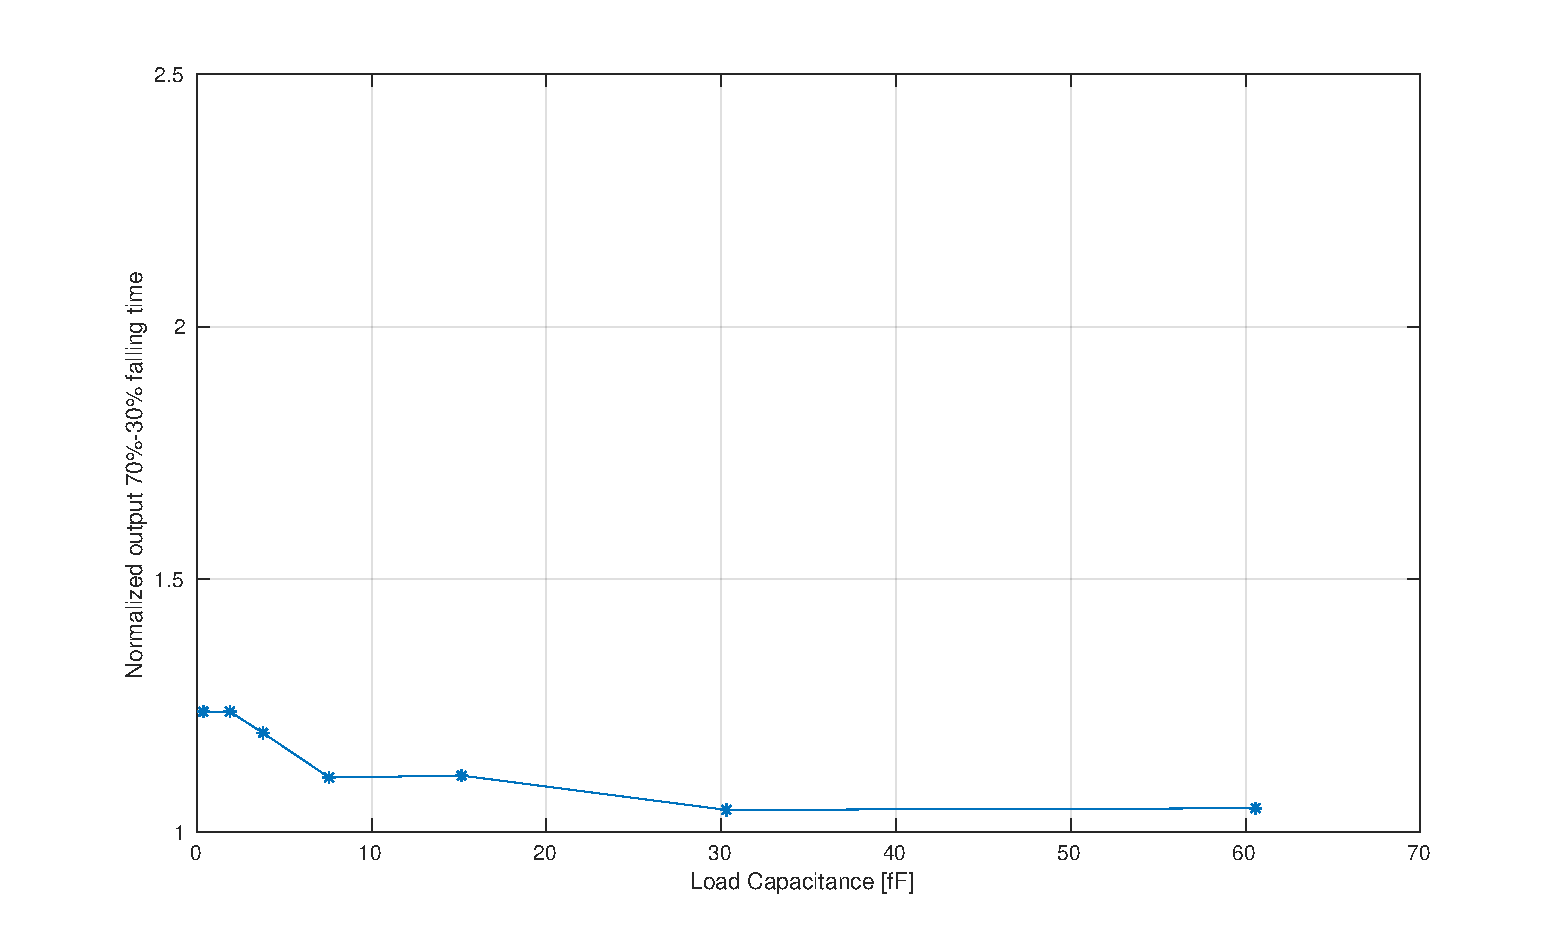
\includegraphics[width=\linewidth]{../INV_X4/simulations/t_F_diff.pdf}
	\caption{Relative fall time difference vs load capacitance}
	\label{fig:inv_t_F_diff}
\end{figure}
\begin{figure}[H]
	\centering
	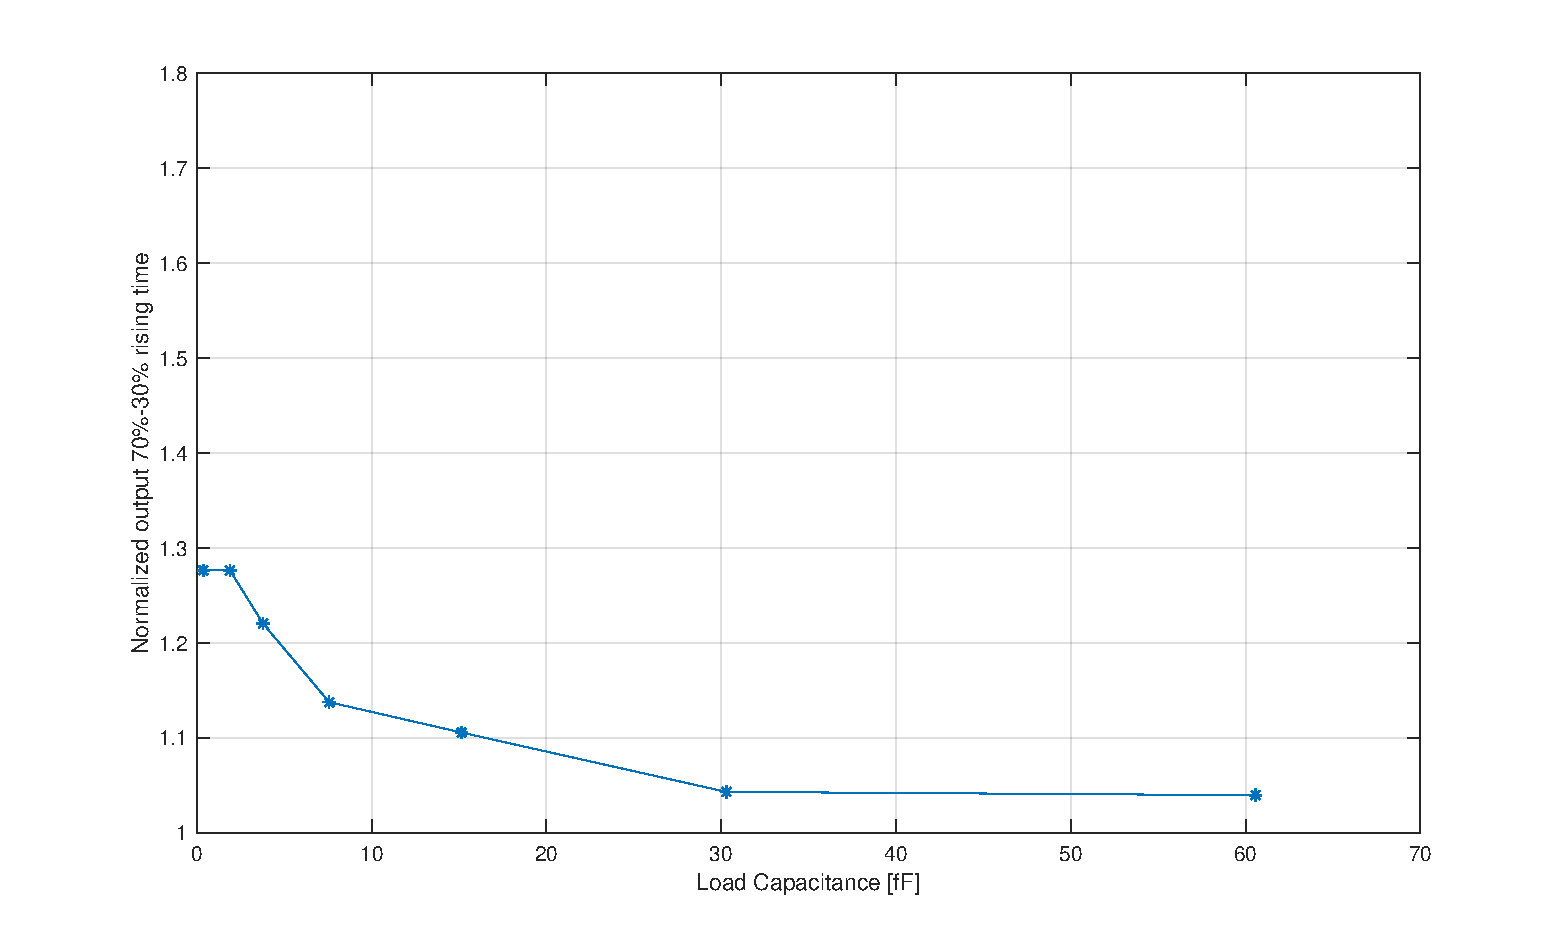
\includegraphics[width=\linewidth]{../INV_X4/simulations/t_R_diff.pdf}
	\caption{Relative rise time difference vs load capacitance}
	\label{fig:inv_t_R_diff}
\end{figure}
\begin{figure}[H]
	\centering
	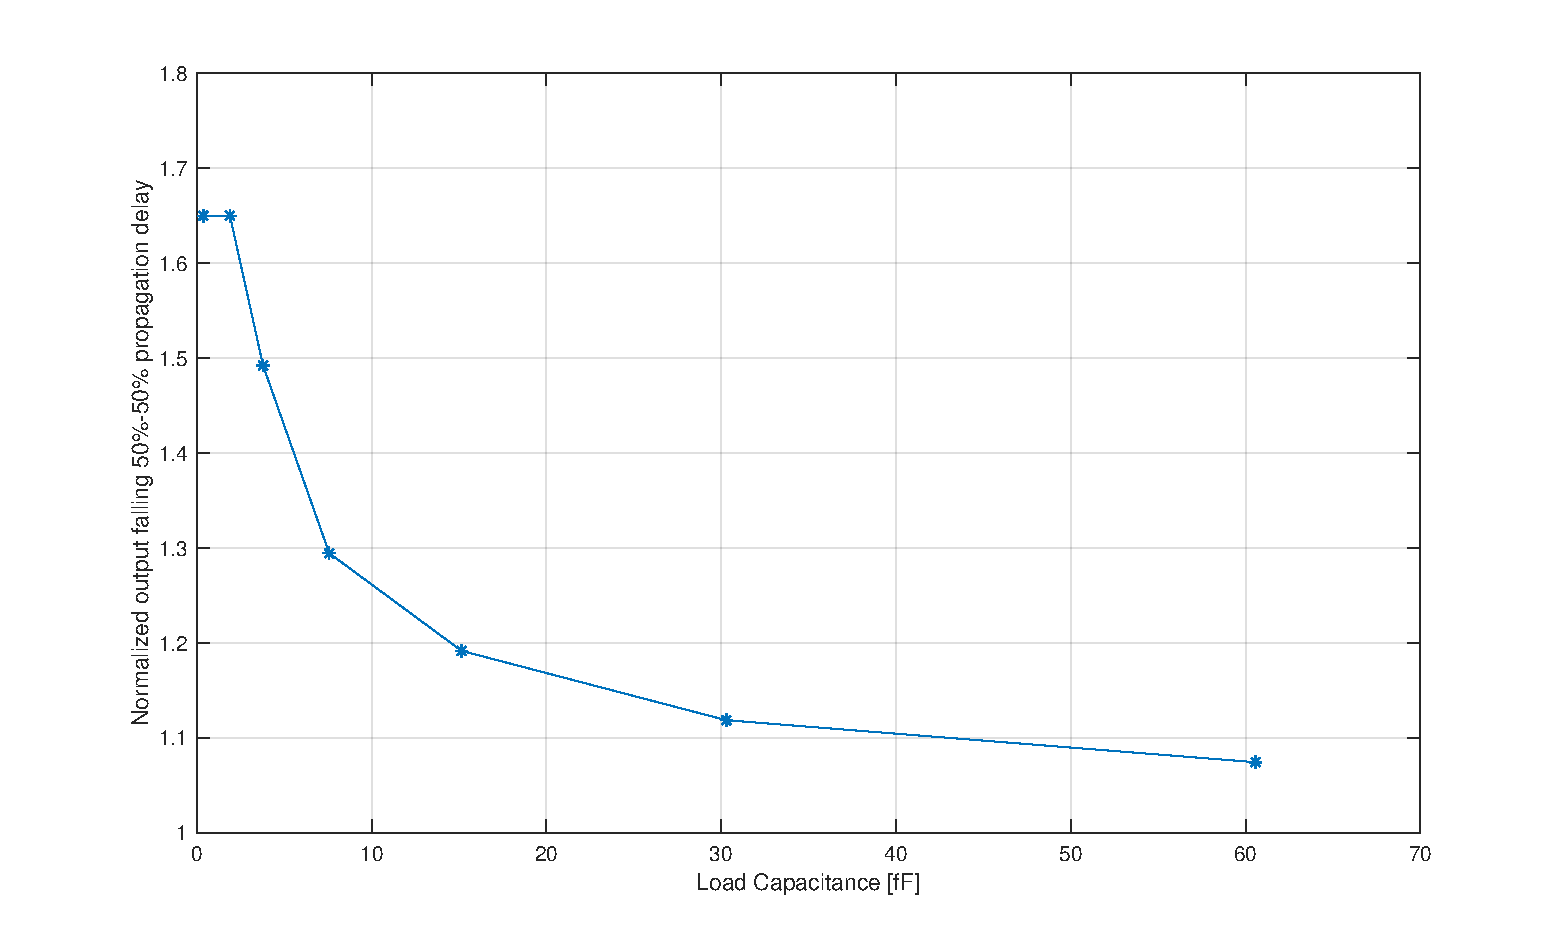
\includegraphics[width=\linewidth]{../INV_X4/simulations/tp_L_diff.pdf}
	\caption{Relative falling propagation delay difference vs load capacitance}
	\label{fig:inv_tp_L_diff}
\end{figure}
\begin{figure}[H]
	\centering
	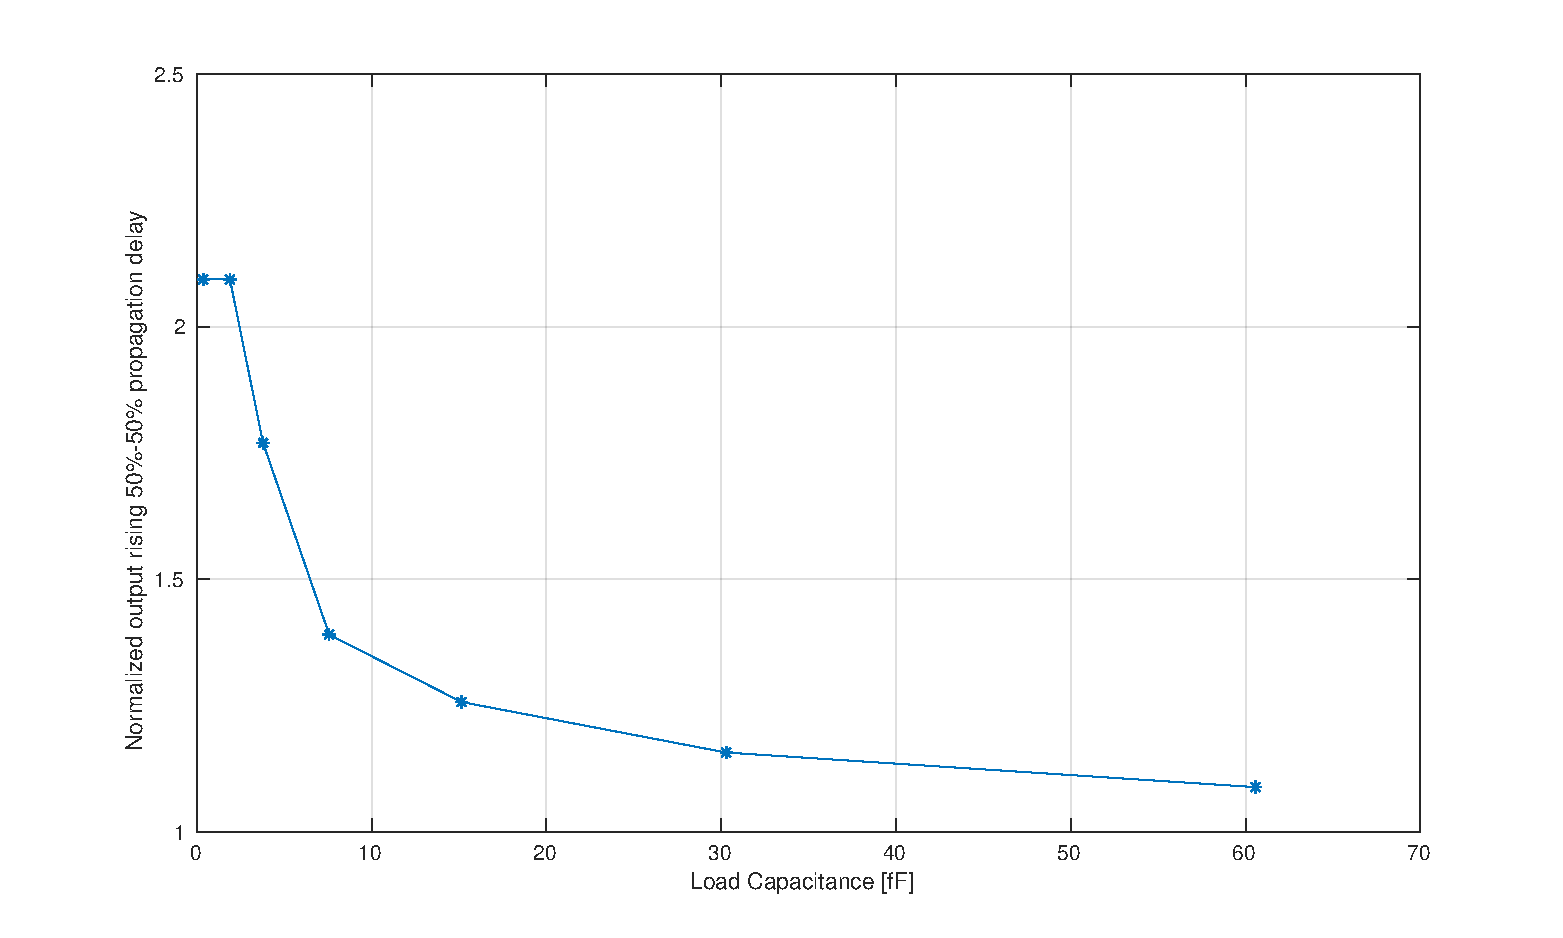
\includegraphics[width=\linewidth]{../INV_X4/simulations/tp_H_diff.pdf}
	\caption{Relative rising propagation delay difference vs load capacitance}
	\label{fig:inv_tp_H_diff}
\end{figure}

We can notice that for very small load capacitance values the simulations done on the extracted parasitics show steadily longer delays, from 20\% to 45\% longer than the schematic-only simulations. This is easily explained by the fact that the parasitic elements have a bigger impact on performance when the load capacitance is very small, while for larger values of load capacitance its effect becomes dominant and the weight of the parasitic contributions drastically reduces.

\newpage
\section{Half adder}
\subsection{Schematic}
The schematic was drawn using Virtuoso Schematic Editor (figure \ref{fig: HAX1_sch}), following the reference \texttt{.png} shown in figure \ref{fig: HAX1_png}.

\begin{figure}[H]
	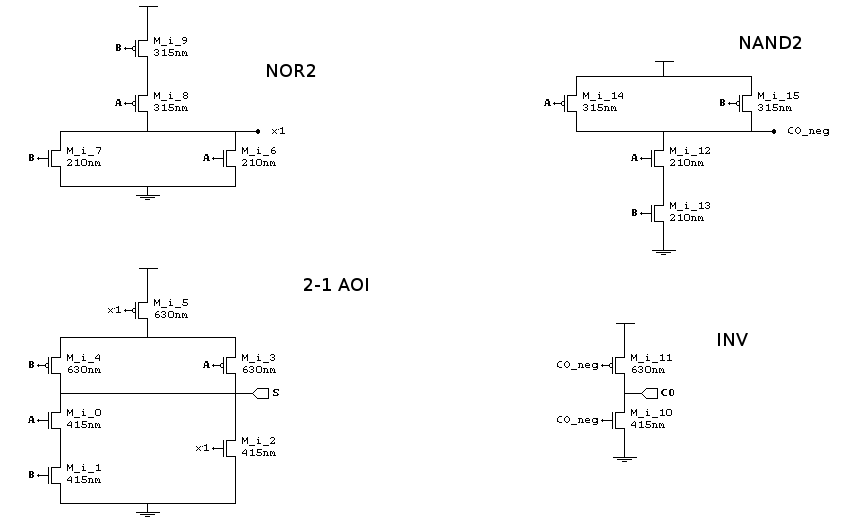
\includegraphics[width=0.9\linewidth]{./Images/HA/HA_X1.png}
	\caption{Reference schematic of the half-adder}
	\label{fig: HAX1_png}
\end{figure}

Even though the AOI21 gate has the pull-up network made of a series PMOS connected through the power supply and two PMOS in parallel, we decided to switch the two subnets to obtain better perfomances. There are two main reasons for this choice:
\begin{enumerate}
\item If A and B are both at '0' and x1 is at '1', the intermediate node is discharged. When a transition of x1 happens then the node has to be charged from only one $R_{eq}$. With two PMOS between the supply and the other transistor the situation could be hypotetically better: in the worst case we could have the same situation as before, but if both A and B are asserted then the capacitance takes less time to complete the charging.
\item The capacitance of the intermidiate node is greater if there are 2 PMOS before the output instead of one.
\end{enumerate}

We report here the final schematic used to create the layout.

\begin{figure}[H]
      \centering
       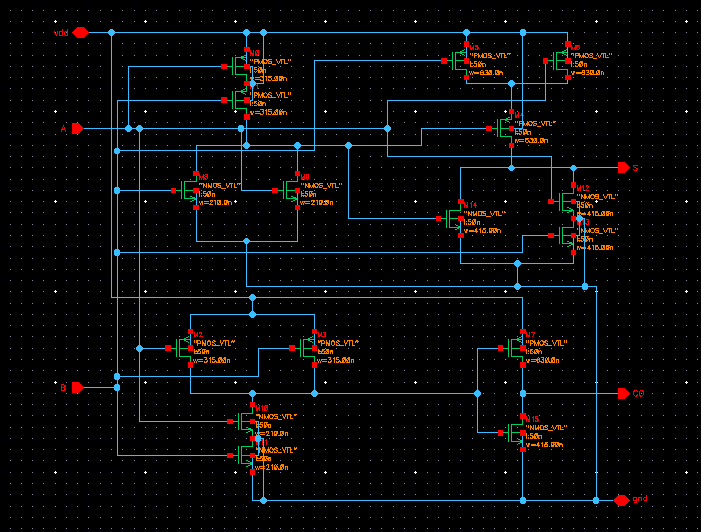
\includegraphics[width=\linewidth]{./Images/HA/HAX1_schematic.png}
\caption{\ha schematic}
\label{fig: HAX1_sch}
\end{figure}

At this point we created a new testbench and we simulated the circuit schematic as we did for the \inv. The cell behaved as it was supposed to. Great!

\begin{figure}[H]
      \centering
       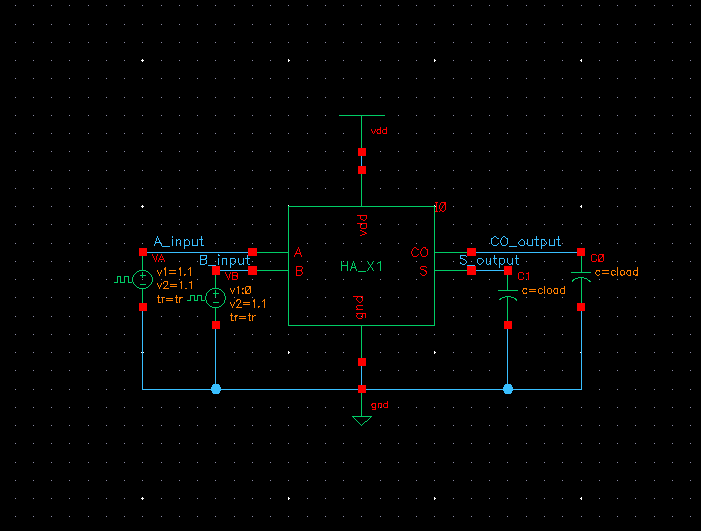
\includegraphics[width=12cm]{./Images/HA/HAX1_TB_schematic.png}
\caption{HAX1 testbench}
\label{fig: HAX1_tb}
\end{figure}

\subsection{Layout}
Given that the layout of the half adder is quite more complex than the one of the inverter, we started by deeply analyzing the possible approaches using the pen-and-paper method. The final solution we came to consisted in sharing source/drain diffusions as much as possible, in order to minimize the area in the horizontal direction, similarly to what we did in the inverter design.

When actually drawing the design in Virtuoso, we made sure to run the Design Rule Checker (DRC) very often, in order to avoid problems in advance. The final result of this tool was totally similar to the one we obtained for the \inv in section \ref{sec: inv_sch}, and thus it is omitted.

The layout design started by looking at the schematic. First of all we tried to put the two outputs on the opposite sides of the cell. This is because this way, if the inputs are brought over it in the middle with the \texttt{metal2} and linked with vias, the input-output paths are more probably balanced in lenght, keeping the input polysilicon lines shorter and therefore reducing these lines' propagation delays. This assumption lead us to place the carry-out generation network (a NAND gate followed by an inverter) on the left of the layout, and the sum generation network (NOR gate followed by an AOI12 gate) on the righ side.
Thus we started drawing on a paper the first NMOS of the inverter whose output was CO. With a view to share the sources/drains as much as possible we began putting all the transistors one near the other drawing only the strictly necessary metal.
We used different colours to have an easier readability and go on drawing only the \texttt{metal1} for the sources/drains and the \texttt{polysilicon} for the gates until the end of the port and left the routing at last. Then we completed the layout linking together the various elements coherently with the schematic view. The resulting pencil draw is reported in figure \ref{fig: lay_drw}.

\begin{figure}[H]
      \centering
      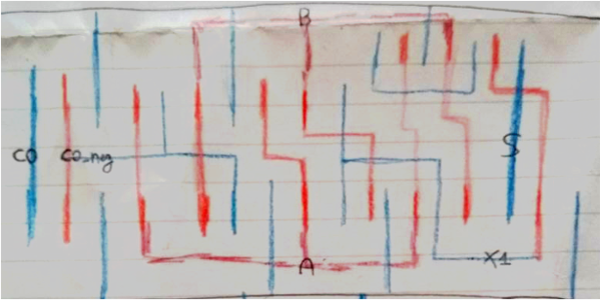
\includegraphics[width=0.8\linewidth]{./Images/HA/layout_drw.png}
	  \caption{First sketch of the layout. \textcolor{blue}{Blue}: metal1, \textcolor{red}{red}: polysilicon. Labels do not match the position of the corresponding vias.}
	  \label{fig: lay_drw}
\end{figure}

Then we converted this sketch in a real layout design using the Virtuoso embedded layout editor. During our sessions we paid attention to reduce every distance to the minimum with the aid of the meter tool and in accordance with the Design Rules. We made a lot of effort to have a cell with the minimum area because the area is directly linked to the yield of the process and to logic ports density, capacitance and therefore delay and power cost per commutation. The less is the area, the more ports can be fitted in a single chip or the more the smaller the chip will be, and it is harder to find defects on a single chip if it is small because the density of the defects per unit area is about constant (higher yield for the process). The delay and the power costs rise with the area because if more material is used, higher resistance/capacitance is added. For this reason we also tried to reduce the length of every wire.

The height of the cell is fixed to \SI{2.66}{\micro\meter} because of the standard-cell format requirements. Its top and ground lines, whose purpose is to power the transistors, are made of \texttt{metal1}. Many entity like this one can be put one next to the other to form a row of cells packed together and fed with global $V_{DD}$ and $GND$ voltage lines.

When we drew the layout with the editor we changed the connections routing a little bit. Instead of putting a single wire of \texttt{polysilicon} to connect each gate with the related input A/B, we used vias and \texttt{metal1} pieces of line. It would have been interesting to compare the performances of the two implementations, to see whether longer polysilicon lines perform better or worse than shorter ones connected through metal lines and vias. Both the layouts are reported in figure \ref{fig: HAX1_layouts}, though only the polysilicon and metal version (figure \ref{fig: polymetal}) has been simulated and characterized due to the lack of time.

\begin{figure}[H]
    \centering
    \begin{subfigure}[h]{\textwidth}
        \centering
        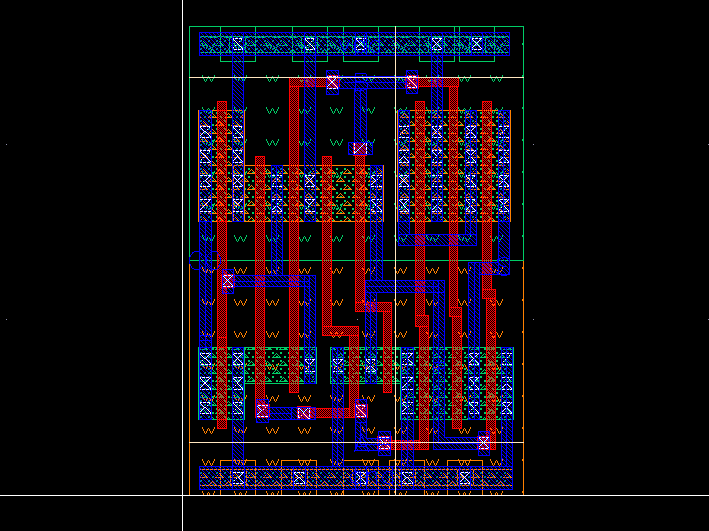
\includegraphics[width=\linewidth]{./Images/HA/HAX1_poly-metal_layout.png}
        \caption{Polysilicon and metal input lines}
		\label{fig: polymetal}
    \end{subfigure}
    \begin{subfigure}[b]{\textwidth}
        \centering
        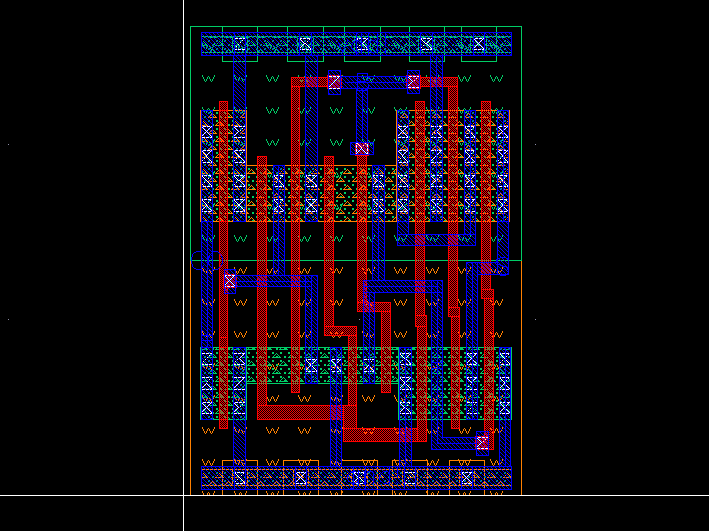
\includegraphics[width=\linewidth]{./Images/HA/HAX1_poly_layout.png}
        \caption{Polysilicon only input lines}
		\label{fig:poly}
    \end{subfigure}
    \caption{Different layouts}
    \label{fig: HAX1_layouts}
\end{figure}

Notice how the final layout in figure \ref{fig: polymetal} appears divided in two different active region both for the NMOS and PMOS networks. This is necessary whenever two metal lines are connected to the active region without a gate between them. In fact, during the manufacturing process, the polysilicon layer is lay before the active one. Therefore, the gates prevent the active regions to extend below them, even if the layout masks do. This automatically isolates the drain and source implants and the related metal lines. When no gate is lay between two metal lines, the isolation must be considered as part of the active layer mask. In the early stages of the development this wasn't clear to us, as proved by figure \ref{fig:poly}.

Finally we launched the LVS and then extracted the parasitic elements. The PEX operation gave us a schematic with all the MOS with the relative parasitics. Again, the output log and schematic listed all the extracted resistances and capacitances similarly to what has been reported for the \inv in section \ref{sec: inv_char}. The net is implicit because no wire is drawn, but every terminal has its own label. The following figures show the group of the 16 MOS of the cell, a detail of one MOS to highlight the labels on the terminals and a parasitic capacitance between the drain of that MOS and \texttt{gnd}.

\begin{figure}[H]
      \centering
       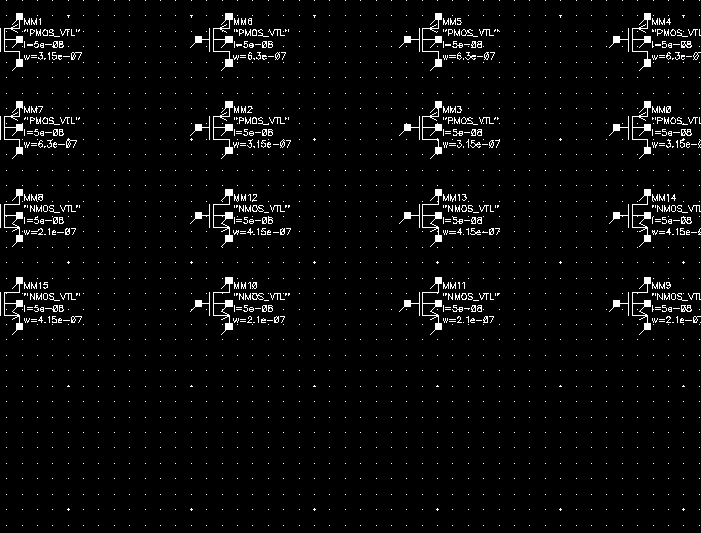
\includegraphics[width=12cm]{./Images/HA/HAX1_PEX.png}
\caption{Detail of the extracted parasitics - group of MOS}
\label{fig: PEX0}
\end{figure}

\begin{figure}[H]
      \centering
       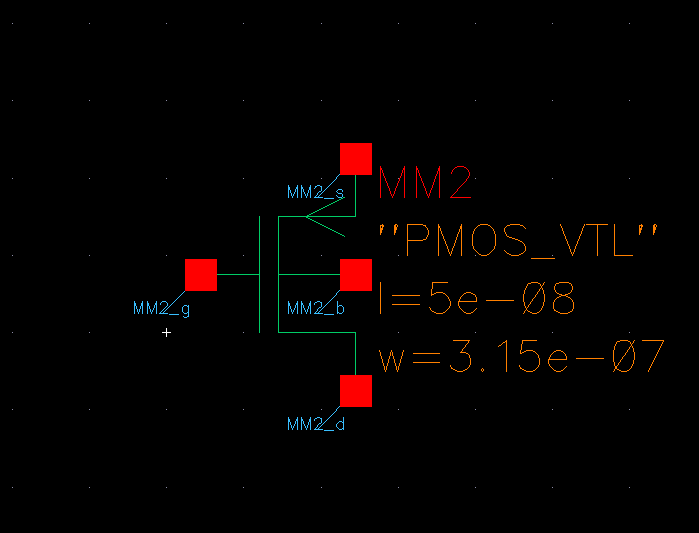
\includegraphics[width=12cm]{./Images/HA/HAX1_PEX_1.png}
\caption{Detail of the extracted parasitics - MOS M2}
\label{fig: PEX1}
\end{figure}

\begin{figure}[H]
      \centering
       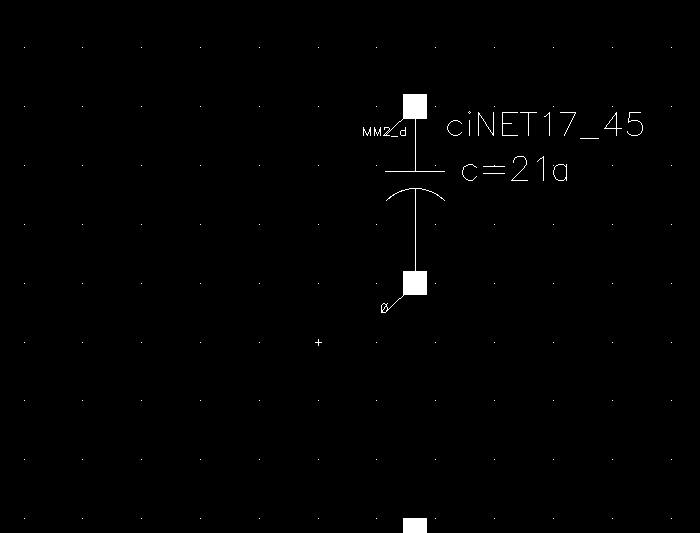
\includegraphics[width=12cm]{./Images/HA/HAX1_PEX_2.png}
\caption{One parasitic capacitance, between the drain of M2 and gnd}
\label{fig: PEX2}
\end{figure}

Every reference can be spotted looking at the schematic and at the relative file. The PEX produced also the report and the netlist files. In the netlist all the informations about the net with the parasitics can be found. For example here we report the part regarding the previous pictures.

\begin{figure}[H]
      \centering
       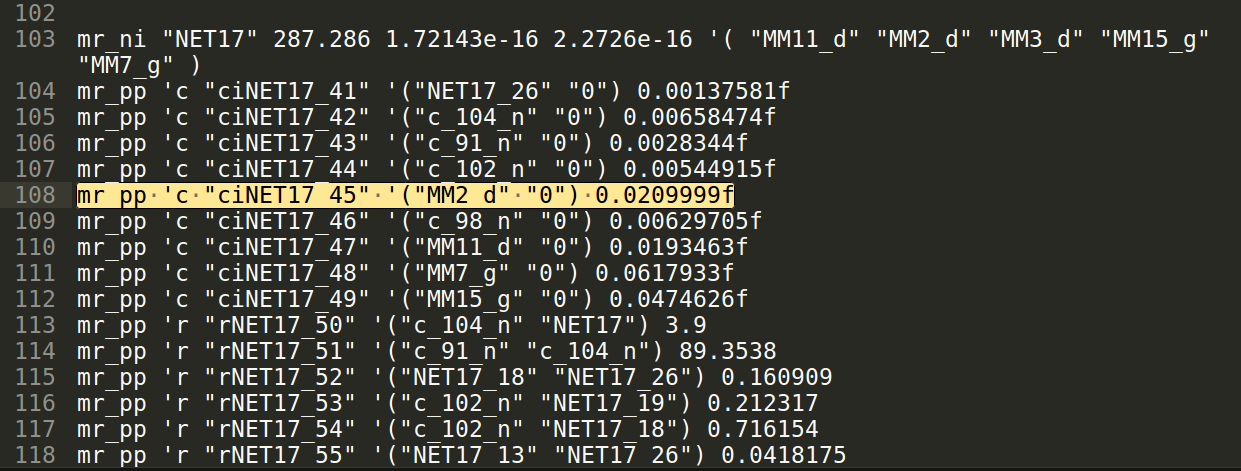
\includegraphics[width=12cm]{./Images/HA/HAX1_PEX_netlist.png}
\caption{Part of the file 'HA-X1.pex.netlist'}
\label{fig: PEX0_netlist}
\end{figure}


\subsection{Characterization}
As done before, we proceeded with the simulation of the layout taking into account the lumped parameters extracted with the PEX tool. From the extracted data we created a new cell configuration (\texttt{config} view) for the \ha. At this point we created a new testbench cell, where we imported our \ha as DUT. Two pulse generators and two load capacitors with parametric values completed the testbench along with the $V_{DD}$ and $GND$ ports.

At this point we were ready to perform the simulations required to fill in the timing characterization tables in the Liberty file. The following simulations are needed:
\begin{itemize}
	\item \textbf{Carry-out} Since the \texttt{CO} generation network is an \texttt{AND} gate of the two inputs \texttt{A} and \texttt{B}, it is necessary to have one of these inputs to be fixed at its high value for the output to switch. Therefore only eight measurements are required to fully characterize this output pin: output falling and rising propagation delays, output fall time and rise time, each of these related to both \texttt{A} and \texttt{B} inputs.

	\item \textbf{Sum} The \texttt{S} generation network is a \texttt{XOR} gate. Its output can thus switch whenever the inputs change from being equal to being different and viceversa. Therefore sixteen measurements are required. It is important to notice that unlike \texttt{CO}, this output shows an inverting behaviour with respect to the related input when the other input is high.
\end{itemize}

Having set properly the measurement parameters in the ADE L simulation environment we ran the parametric simulation with the same input transition times and load capacitance values used for the \inv.

Only the results regarding the output falling propagation delays and the output fall times related to the \texttt{A} input are reported. The output rising propagation delays and output rising time are slightly higher than these, of about \SIrange{10}{20}{\nano\second}, but the behaviour is completely similar. Since the \texttt{A} and \texttt{B} paths are quite balanced, there's almost no difference betweeen the related timing parameters. Therefore they are omitted for the sake of clarity and mercy for the reader. Instead, both the measurements related to \texttt{CO} and \texttt{S} are reported one next to the other, in order to make the comparison easier. In figure \ref{fig:HA_tp_L} the output falling propagation delays are shown, while the falling transition times can be found in figure \ref{fig:HA_t_F}.

\begin{figure}[ht]
	\centering
	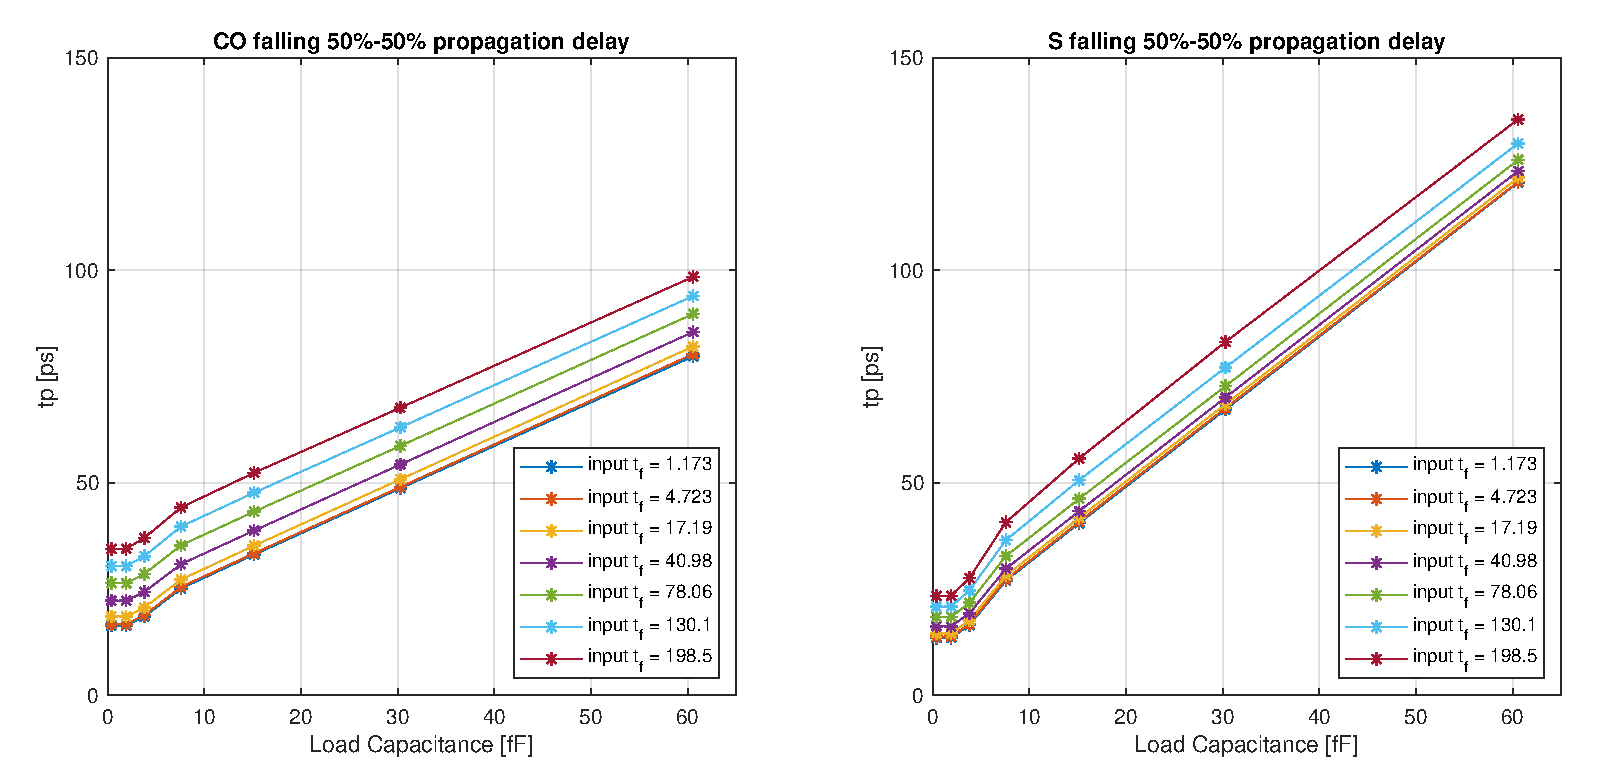
\includegraphics[width=\linewidth]{Images/HA/tp_L_crop.pdf}
	\caption{\ha output falling propagation delays}
	\label{fig:HA_tp_L}
\end{figure}

\begin{figure}[ht]
	\centering
	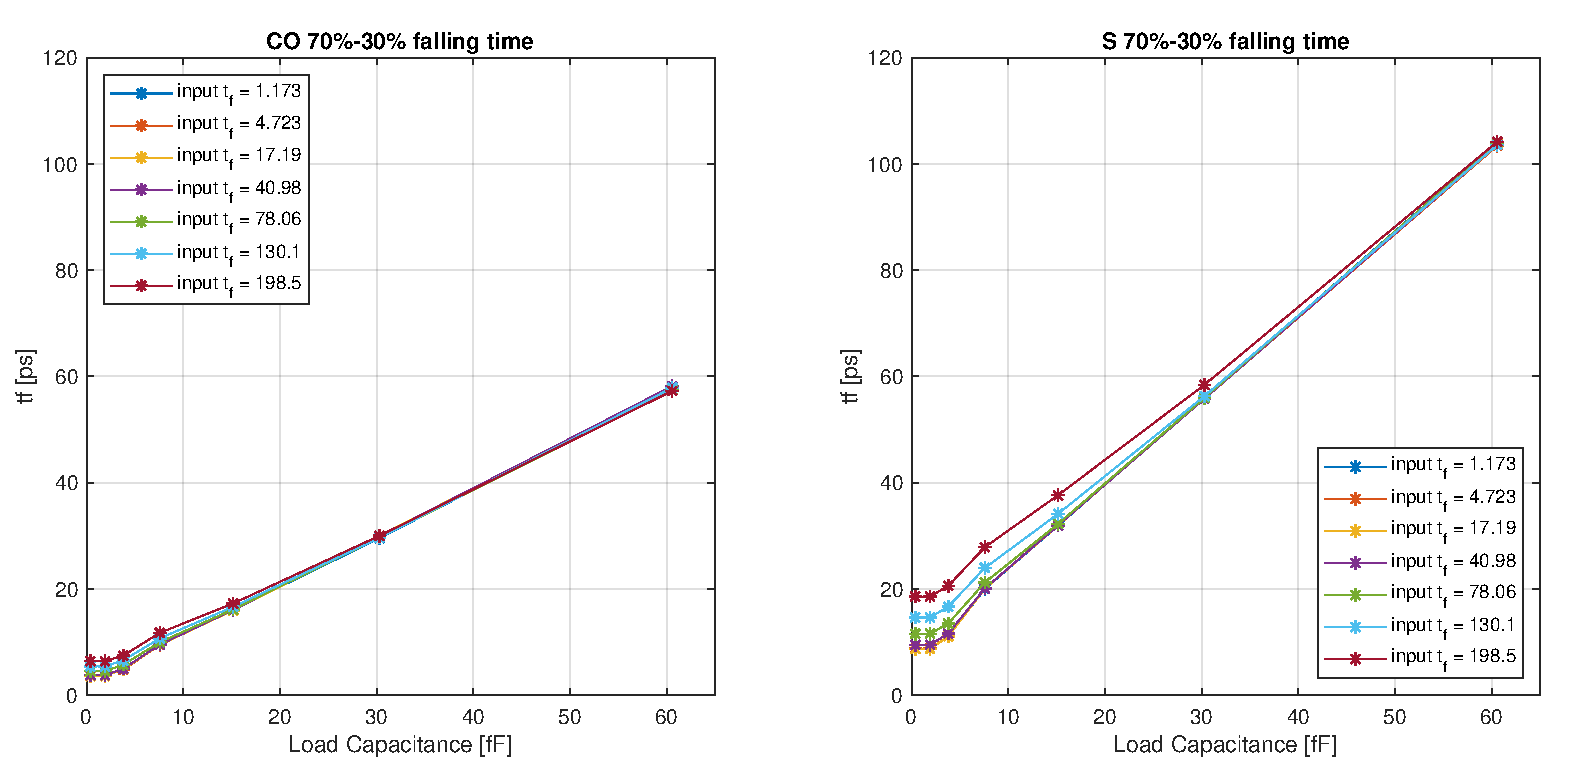
\includegraphics[width=\linewidth]{Images/HA/t_F_crop.pdf}
	\caption{\ha output falling times}
	\label{fig:HA_t_F}
\end{figure}

The propagation delay of \texttt{S} is lower than the one of \texttt{CO} for very low input transition time and low load capacitance, while it becomes higher at higher values of load capacitance. This behaviour can be explained taking a look at the transistor widths of the two output generation pulldown networks. These are not completely optimized, since two transistors in series have the same width as one transistor alone (see for example the \texttt{AOI12} gate in figure \ref{fig: HAX1_sch}). On the other side, since the inverter in CMOS technology is the logic gate with the higher capacitive gain, the \texttt{CO} generation network is supposed to behave better (lower delays) with higher loads. This is also true for the output transition times, as shown in \ref{fig:HA_t_F}. Another conclusion can be reached from this second plot is that the input transition time has a greater impact with low load capacitances, while for higher values the slope of the output signals is mainly determined by this last component, as confirmed by the converging curves and by the \inv analysis discussed before.

Having done the characterization of the \ha on the basis of its lumped parameters from the designed layout, we are intrested in seing how these affect its behaviour with respect to the schematic-based transistor model. This purpose is better achieved with 3D plots, that can easily show the relation among delay, input transition times and load capacitance. These plots are reported in figure \ref{fig:HA_tp_L_diff} and \ref{fig:HA_t_F_diff}.

\begin{figure}[ht]
	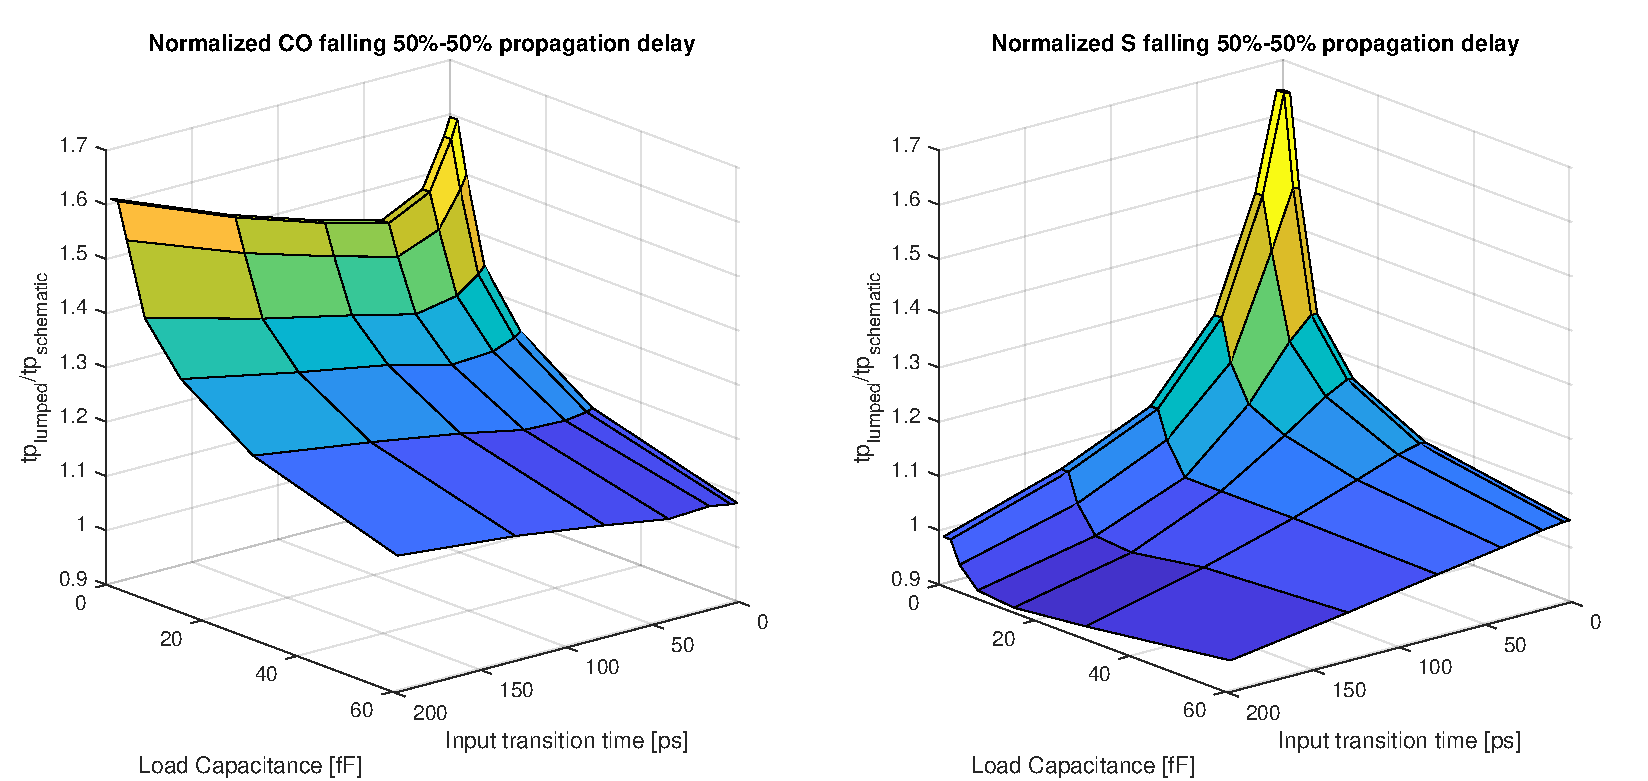
\includegraphics[width=\linewidth]{Images/HA/tp_L_diff_crop.pdf}
	\caption{Relative output falling propagation delays vs. load capacitance and input transition time}
	\label{fig:HA_tp_L_diff}
\end{figure}

\begin{figure}[ht]
	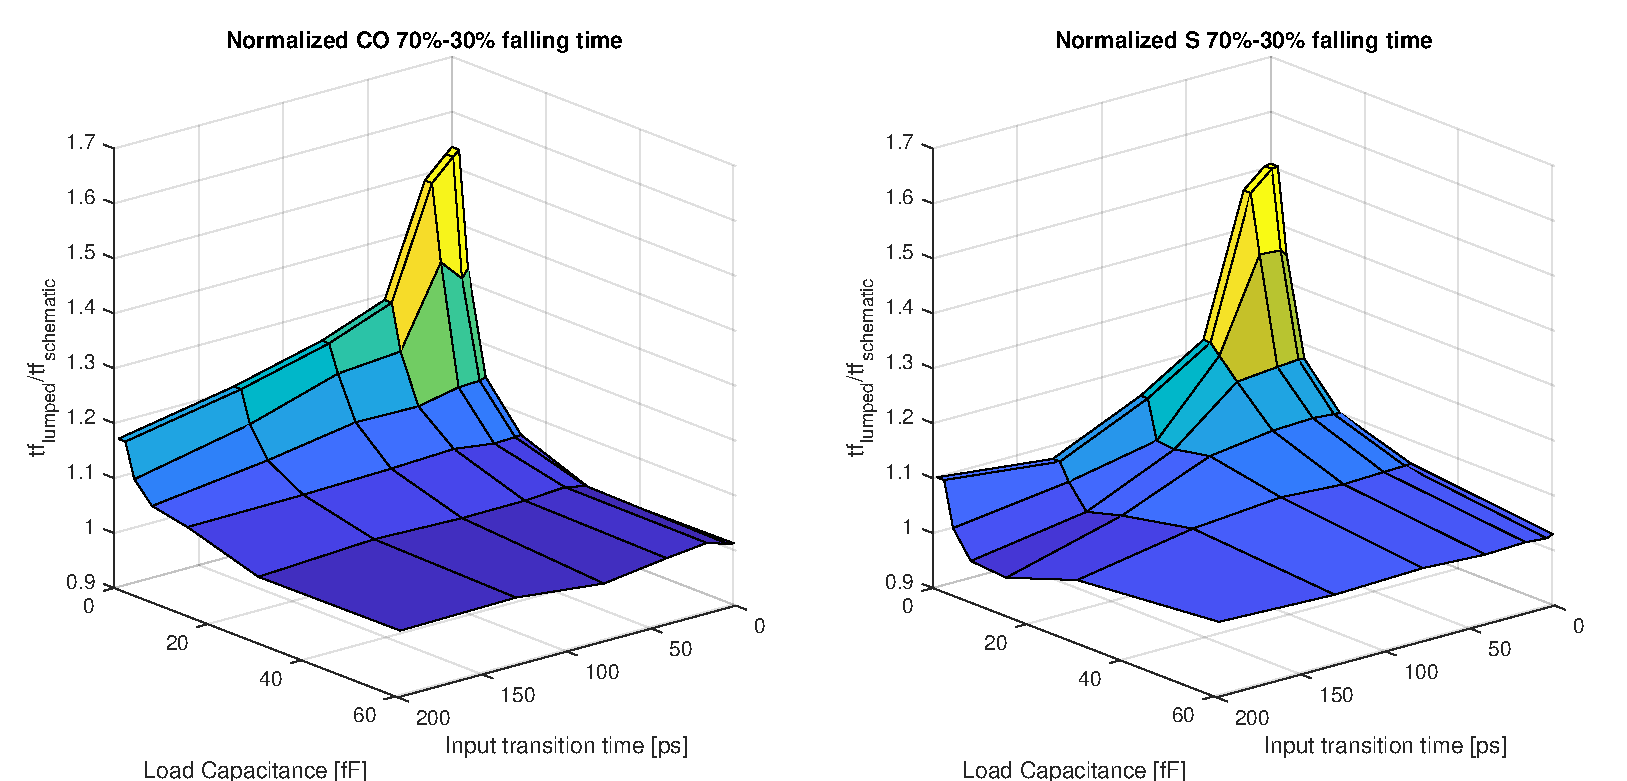
\includegraphics[width=\linewidth]{Images/HA/t_F_diff_crop.pdf}
	\caption{Relative output falling times vs. load capacitance and input transition time}
	\label{fig:HA_t_F_diff}
\end{figure}

As we expected, the impact of the lumped components is much grater at lower load capacitances and shorter input transition times, where the timing parameters are about 60\% greater. However, it is intresting to observe how different this impact is when comparing the two output networks. For \texttt{CO} the propagation delay increases with the load capacitance, while it decreases for \texttt{S}. This latter case leads the difference to become even negative at the highest load capacitance and lower input transition time (ratio $tp_{lumped}/tp_{schematic} < 1$), where the lumped parameters simulations brought better timing performance with respect to the schematic ones. The reason for this is uncertain, but it can be related to the shared sources and drains of the different transistors, that could lead to overall lower lumped capacitance with respect to the ones taken into account by the schematic simulation models.

If we look at the plots, we can also see how there's no difference between the simulations at the lowest two values of the input signal transition times. This may be due to the simulation resolution.

\subsection{Remarks}

\begin{itemize}
	\item \textbf{Working frequency} From the timing parameters (see the file \texttt{HA\_X1.lib} for full characterization) we can see how the propagation delay of the \ha is always lower than \SI{150}{\pico\second}. This means that the component can be inserted in a circuit (for example a pipeline stage) that works at a maximum clock frequency of \SI{6.7}{\giga\hertz}, if sequential components timing constraints are ignored.
\end{itemize}

\section{Conclusions}
\begin{itemize}
	\item \textbf{Area} Due to the different input vector used for the characterization of the original library gates it is impossible to directly compare those cells with ours. However, a comparison can be done about the standard cell areas. The standard cell like design fixes the height of the gates to \SI{2.67}{\micro\meter} for both the layouts.
	\begin{itemize}
		\item For the \inv we were able to achieve a cell width of \SI{1.33}{\micro\meter}, slightly larger than the \SI{1.0975}{\micro\meter} of the original layout.

		\item For the \ha we managed to achieve much better results, resulting in a width of \SI{1.9025}{\micro\meter} versus the \SI{2.66}{\micro\meter} of the original layout.
	\end{itemize}

	\item \textbf{Further optimization} Better timing performance and smaller areas could be obtained changing the reference design transistor widths according to the best solution for the specific maximum load, setting every single gate width in order to balance the logical effort and driving strength. Nevertheless in this instance we focused on a first level optimization through source/drain sharing and metal/polysilicon paths routing. The use of \texttt{metal1} only makes it possible to employ the upper metal levels to realize the interconnections betweeen cells.
\end{itemize}

\end{document}
